\section{Experimental Evaluation}
\label{eval}

\subsection{Datasets and evaluation protocol} \label{eval:protocol}
Our default dataset in this paper will be INRIA \emph{Holidays} dataset \cite{holidays}. This dataset consists of 1491 images divided in 500 groups of matching images. For the remaining of this report, if the dataset of an experiment is not mentioned, the experiment is performed on \emph{Holidays}.
We also perform in the \emph{Oxford} dataset \cite{oxford}, which consists of 5062 images separated in 55 groups of matching images.

Each group of these datasets contains one query image. 
For each query image, we calculate its similarity to all other images in the database and rank them, in decreasing order. 
The average precision of a group is calculated by the ranking of the images of the group for the similarity with the corresponding query image. 
The final mean average precision (mAP) for a dataset is the mean of the average precision over all its groups.
As negative sample of images, we use a set of images $10^5$ from Flickr \cite{oxford}. 
For a full rank decomposition, we use a subset of Flickr100k, between $6000$ and 15000 images. 
As stated in section \ref{low-rank} and further discussed in section \ref{time-scale}, a full rank decomposition does not scale well for bigger number of negative samples. For low rank decomposition, we use all 100000 images.

At evaluation time, for a dataset that consists of $p$ images and $q$ query images, we calculate its $p\times q$ \emph{similarity matrix} $S$, where each of its $q$ columns is the matching scores of the query image with all the $p$ images.


\subsection{Which kernel to choose?}
We tested four different kernels: linear kernel, RBF kernel, polynomial kernel and spatial pyramid match kernel. Each kernel takes as parameter a scalar $\gamma$.

\begin{align}
    &k_{linear}(x,y) = x^Ty; \label{k:lin}\\
    &k_{rbf}(x,y) = \exp(-\gamma|\! |x-y|\! |^2); \label{k:rbf}\\
    &k_{poly}(x,y) = x^Ty+\gamma(x^Ty)^2; \label{k:poly}\\
    %&k_{spp}(x,y) = \dfrac{1}{2^L}\mathcal{I}(H^0_x, H^0_y) +\sum_{l=1}^L\dfrac{1}{2^{L-l+1}}\mathcal{I}(H^{l,\gamma}_x, H^{l,\gamma}_y). \label{k:spm}
\end{align}
\textbf{Linear SLEM} The linear kernel of Equation (\ref{k:lin}) is the first default choice and equivalent to the non-kernelized version of SLEM.
In the remaining of this paper, we reference to linear SLEM when we use the non-kernelized SLEM.
\textbf{Gaussian SLEM} The radial basis function kernel of Equation (\ref{k:rbf}) is a
well known reproducing kernel, used for classification with support vector machines.
\textbf{Polynomial SLEM} The polynomial kernel of Equation (\ref{k:poly}) is a reproducing kernel normally used in natural language processing. 
%\textbf{SPM SLEM} The spatial pyramid matching kernel of $L+1$ levels in Equation \ref{k:spm} take as input a set of local descriptors and its location in pyramidal bins \cite{spk}. 


\subsection{Base visual features}
We test our feature encoder for two different features, one hand-crafted image representation and one learned from deep convolutional neural networks.


We revisit the VLAD feature presented in \cite{VLAD} as an example of a hand-crafted representation. First we extract a set $\mathcal{F}$ of local descriptors of an image $I$. We use the 128 dimension RootSIFT \cite{3things} descriptors, extracted densely. 
Then, we hard-assign each descriptor $f$ in $\mathcal{F}$ to one of $K$ set $\mathcal{C}_k$ of descriptors associated to codewords $\{c_k\}_{1\leq k\leq K}$, and map $f$ a $\RR^{128K}$ vector 
\begin{equation}
\phi^{VL}_1(f) = \left[0 \ 0 \ 0 ..., \Phi_k^T\frac{(f-c_k)}{||f-c_k||},... 0\right],
\end{equation}
where $\Phi_k$ is the $128\times 128$ PCA matrix associated to descriptors in $\mathcal{C}_k$. 
The final VLAD representation is the power-normalization and $l_2$ normalization of the sum-pooling of $\phi^{VL}_1$:
\begin{equation}
\phi^{VL}_2(I) = \sum_{f\in \mathcal{F}}\phi^{VL}_1(f).
\end{equation}
In this paper, we use $K=64$ codewords learned in images from Flickr. Our VLAD representation has 8192 dimensions.

Convolutional features obtained from very deep neural networks have been shown to work as good matching local descriptors \cite{SimonZisser15}. 
The SPoC representation \cite{babenko15} is a weighted sum-pooling of the activations of the last convolutional layer of a 19 layer convolutional neural network. 
Indeed, if our last convolutional layer has $D$ neurons, and each neuron a $W\times H$ map of activations of this neurons to the image $I$, 
each pair $(w,h)$ with $w$ in $\{1,2,..., W\}$ and $h$ in $\{1,2,...,H\}$ can be associated to a descriptor $f_{(h,w)}$ in $\RR^D$ of the responses of each neuron at coordinate $(w,h)$ of the maps. 
We then sum-pool the descriptors $f_{(w,h)}$ weighted accordingly to its distance to the center of the image:
\begin{equation}
    \phi^{SPoC}(I) = \sum_{w=1}^W\sum_{h=1}^H \alpha_{(w,h)}f_{(w,h)},
\end{equation}
where
\begin{equation}
    \alpha_{(w,h)} = exp \left(-\dfrac{(w-W/2)^2+(h-H/2)^2}{2\sigma^2}\right).
\end{equation}

%We use four base features as the representation in $\RR^d$ of our images. Firstly, we use VLAD features, as used in \cite{ZePe15}. 
%CNN features are non-negative and can be used both as $\mathbb{L}^1$ or $\mathbb{L}^2$ normalized features. The third features are spatial pyramids of SIFT descriptors, as used in \cite{spk}. These are non-negative $\mathbb{L}^1$ normalized features. \emph{\color{red} Details of these features construction are not relevant right now.}


\subsection{Implementation details}
\emph{\color{red} Not relevant right now.  To be written.}
$8192$ dimensional VLAD features.

E-SVM: $0.6$ second to solve one single exemplar.

SLEM: $30$ seconds to solve a $8192\times 8192$ linear system for all exemplars of the dataset.

Kernelized SLEM: at most $0.3$ seconds (for RBF kernel) for each iteration of (\ref{icd:algo}) algorithm plus at most $30$ seconds to solve a $r'\times r'$ system.


\subsection{Full rank results}

\begin{table*}[t]
\begin{center}
\begin{tabular}{|c|c|c|c|c|c|}
\hline
Method, features & VLAD-64 \cite{VLAD}& SPoC CNN \cite{babenko15} &  SP-CNN \cite{SPPCNN} \\
\hline\hline
Baseline            & 72.7  & 73.1 & 64.7\\
%Whitening           & -    & -    & -    & -    & -\\
LDA                 & 69.4 & 77.5 & -\\
E-SVM               & 77.5 & 79.8 & 64.7 \\
Linear SLEM         & 78   & 78.3 & 68 \\
Gaussian SLEM       & 78.1 & 81.4 & 68.6 \\
Poly SLEM           & 78.1 &  82   &   -   \\
\hline
\end{tabular}
\end{center}
\caption{Mean average precision results for INRIA Holidays dataset, expressed as percentages. The - means the tests can not be performed or was not performed yet.}
\end{table*}


\begin{table*}[t]
\begin{center}
\begin{tabular}{|c|c|c|c|c|c|}
\hline
Method, features & VLAD-64 \cite{VLAD} & SPoC CNN \cite{babenko15} &  SP-CNN \cite{SPPCNN} \\
\hline\hline
Baseline            & 46.3 & 54.4 & 44 \\
%Whitening           & 07   & 20.2 & - & -    & -\\
LDA                 & 50.9 & 63.7 & 37.4\\
E-SVM               & 57.5  & 62.1 & - \\
Linear SLEM         & 57.5  & 64.1 & 45 \\
Gaussian SLEM       & 59    & 64.9 & 45 (no cv) \\
\hline
\end{tabular}
\end{center}
\caption{Mean average precision results for Oxford 5k buildings dataset, expressed as percentages. The - means the tests can not be performed or was not performed yet.}
\end{table*}


\subsection{Time Scalability} \label{time-scale}
In this section we compare the time efficiency of our method and the E-SVM, as well as discuss which method to use accordingly with the number of positive and negative samples.

We test both methods for $n=6000$ and $n=15000$ negative samples. It is important to note that, since ESVM is optimized by a stochastic gradient descent, its time calculation depends linearly on the number of iterations $T$ it takes to the cost function to converge. We follow the instructions of \cite{ZePe15} and set $T=10000$ for $n=6000$ and $T=100000$ for $n=15000$.
\begin{figure}[!h]
\centering
\begin{subfigure}[b]{0.32\textwidth}
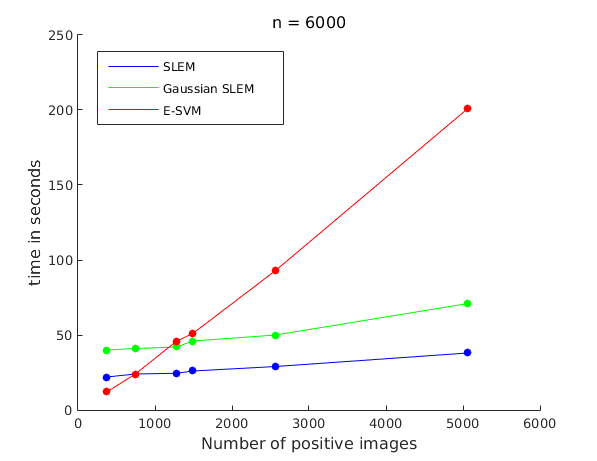
\includegraphics[width=\textwidth]{speed_n_6K.png}
\end{subfigure}
\begin{subfigure}[b]{0.32\textwidth}
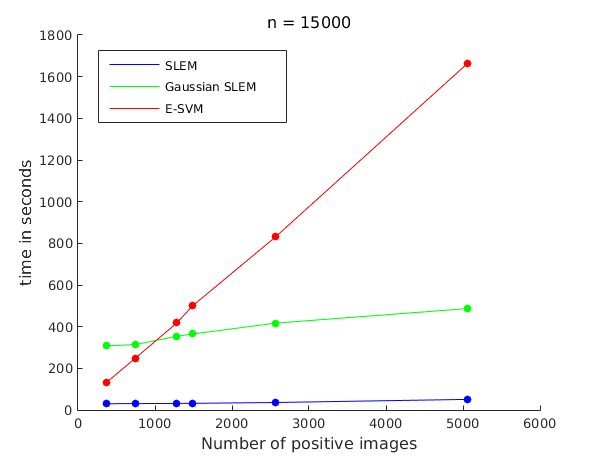
\includegraphics[width=\textwidth]{speed_n_15K.png}
\end{subfigure}
\begin{subfigure}[b]{0.32\textwidth}
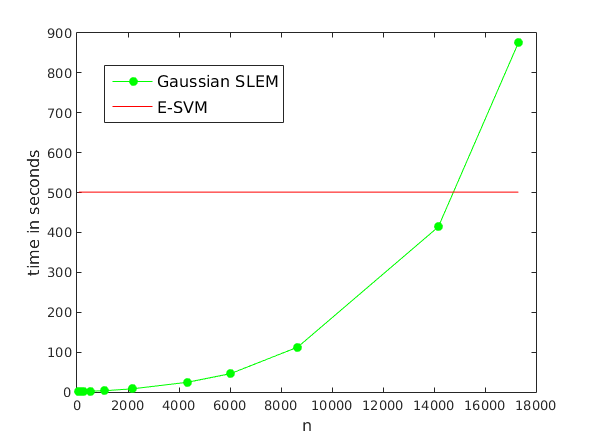
\includegraphics[width=\textwidth]{speed_n.png}
\end{subfigure}
\caption{Comparison between time calculation feature encoding for different methods. At left, we use $n=6000$ negative examples. At right, $n=15000$ negative examples. In both experiments, we use VLAD as base features.}
\label{time:scalar}
\end{figure}
Figure \ref{time:scalar} show how SLEM and ESVM scale for different number of images. Time calculation for ESVM increases linearly with the 

\subsection{Low-rank decomposition evaluation}

\begin{figure}[!h]
\centering
\begin{subfigure}[b]{0.48\textwidth}
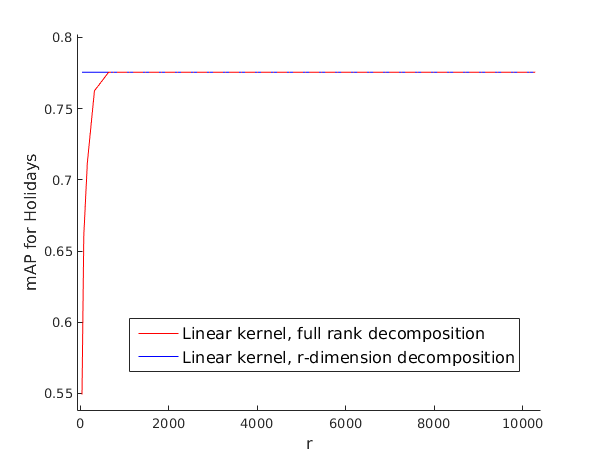
\includegraphics[width=\textwidth]{linear_decomposition_nolog.png}
\end{subfigure}
\begin{subfigure}[b]{0.48\textwidth}
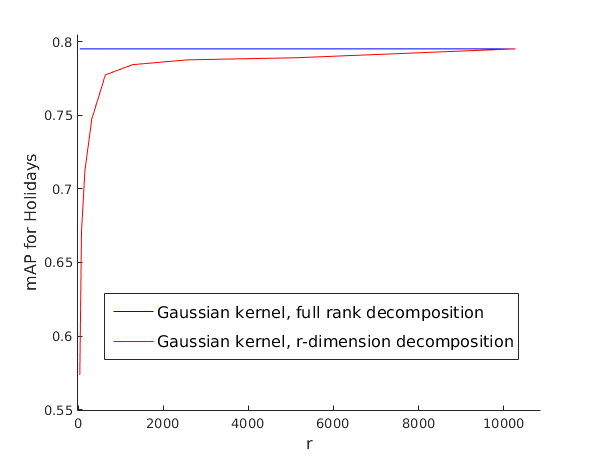
\includegraphics[width=\textwidth]{rbf_decomposition_nolog.png}
\end{subfigure}
\caption{Comparison between full rank and low rank. In blue, mAP results for full rank SLEM. In red, mAP results for low rank decomposition of SLEM, varying the rank $r'$.
At the left, linear SLEM results;at the right, Gaussian SLEM results. In this experiment, $n=10281$.}
\label{no.ker.vs.linear2}
\end{figure}

\subsection{Recursive SLEM}
%\caption{Comparison between no kernel results and linear kernel results. In black, mAP of non kernelized SLEM. In red, mAP for different low-rank decompositions of linear kernel matrix. In this experiment, $r=2^{13}$ and we set $\log_2 r'$ in $\{6, 7,...,13\}$. }

%\caption{Comparison between no kernel results and linear kernel results. In black, mAP of non kernelized SLEM. In red, mAP for different low-rank decompositions of linear kernel matrix. In this experiment, $r=2^{13}$ and we set $\log_2 r'$ in $\{6, 7,...,13\}$. }


